\documentclass[12pt]{article}
\usepackage{graphicx}
\usepackage{amsmath}
\usepackage{amssymb}
\usepackage{color}
\usepackage{caption}
\usepackage{subcaption}
\usepackage{mdframed}
\usepackage[margin=3cm]{geometry}
\usepackage[superscript,nomove]{cite}
\numberwithin{equation}{section}
\numberwithin{figure}{section}
\usepackage[makeroom]{cancel}
\usepackage{textcomp}
\usepackage{gensymb}
\DeclareMathOperator\arctanh{arctanh}
\usepackage[colorlinks=true]{hyperref}
\usepackage{cleveref}
\crefdefaultlabelformat{[#2#1#3]}
\begin{document}
\renewcommand\citeform[1]{[#1]}
%
\title{MSc Data Science Proposal: Can a Convolutional Neural Network judge a book by its cover?}
\author{\\Ryan Hill MSci\\\\
Supervisor: Dr Hubie Chen\\\\
Birkbeck, University Of London\\\\
\texttt{rhill06@mail.bbk.ac.uk}}
\date{\today}
\maketitle
\thispagestyle{empty}
\graphicspath{{images/}}
\begin{abstract}
	In this work we make a proposal for training convolutional neural networks to predict the genre of a book, based on its cover. We evaluate the prior work done in this area and the proposed improvements of the existing dataset known as \emph{BookCover30}. We break the work into 3 stages and provide detail on the proposed hardware and software usage within the project.
\end{abstract}
\begin{figure}[!b]
	\centering
	
\includegraphics[scale=0.4]{bbk_logo.jpg}
\end{figure}

\clearpage
%
{\hypersetup{linkcolor=black}
\tableofcontents}
\thispagestyle{empty}
\clearpage
%
\setcounter{page}{1}
\section{Introduction} % (fold)
\label{sec:intro}
\subsection{Background} % (fold)
\label{sub:background}
\emph{Don't judge a book by its cover} is a common English idiom, with its origin somewhere around the mid 19\textsuperscript{th} century, often cited as being from the newspaper \emph{Piqua Democrat} as follows:
\begin{quote}
	``Don’t judge a book by its cover, see a man by his cloth, as there is often a good deal of solid worth and superior skill underneath a jacket and yaller pants.''
\end{quote}
The phrase itself refers to the idea that one should not judge an item, or person, by how it first appears, but instead you should take the time to understand it better. That being said, a huge amount of cost and effort can go into the design and choice of a cover for a book; costs for cover design alone can range from a few dollars to a few thousand \cite{AdriasG}, and revenue from publishing in 2018 was around \$122bn \cite{Watson}. This value, combined with the fact that humans have been shown to make judgments within 100ms of exposure to another person \cite{Willis2006}, means it is reasonable to assume that this advice is not often taken literally and that as humans we do, in fact, judge a book by its cover.

Beyond the focus of the judgement placed on book covers, they are designed to help the potential reader understand the type of story, or contents, a book may contain. As an example, consider the covers shown in \cref{fig:2bookcovers} that should, even if they had no words on them, help the reader identify immediately the type of content contained within. The type of this content is what we refer to as the \emph{genre} of the book. Even within this example it is clear that there could be some subjectivity, as the reader you may see a dragon and assume it is a fantasy novel, but the Teen \& Young Adult genre often encompasses many genres just due to the age of the intended audience. 
\begin{figure*}[t!]
    \centering
    \begin{subfigure}[t]{0.5\textwidth}
        \centering
        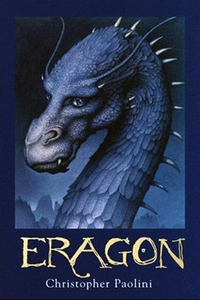
\includegraphics[width=.8\linewidth]{200px-Eragon_book_cover.png}  
	  \caption{Cover of Eragon, Teen \& Young Adult Genre}
    \end{subfigure}%
    ~ 
    \begin{subfigure}[t]{0.5\textwidth}
        \centering
        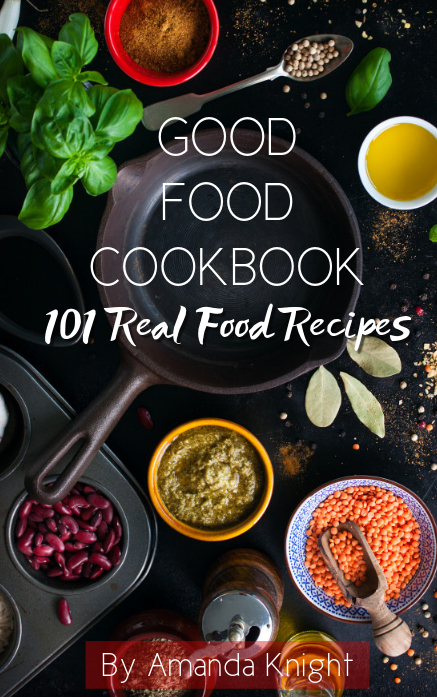
\includegraphics[width=.8\linewidth]{cookbook_cover.jpg} 
	  \caption{Cover of Good Food Cookbook, Cookbooks, Food \& Wine Genre}
    \end{subfigure}
	\caption{Two book covers with distinctly different designs and genres}
	\label{fig:2bookcovers}
\end{figure*}

% subsection background (end)
\subsection{Problem Statement} % (fold)
\label{sub:problem_statement}
In this work we will try to answer one seemingly simple question; \emph{can a Convolutional Neural Network predict the genre of a book based solely upon an image of the front of the book?} Or put another way, \emph{can a Convolutional Neural Network judge a book by its cover?} This may seem like a fairly simple question, but in many cases it might already be quite difficult for a human to distinguish which genre a given book belongs to as just discussed. Beyond answering this question we will also attempt to take the easiest and hardest to identify genres (as determined by the accuracy of the classifier) and use feature visualisation to generate ideal covers for these genres, as the Convolutional Neural Network \emph{sees} them.

The rest of this work is structed as follows; first we review the existing literature and history of computer vision, predicting genre from book covers, and feature visualisation in \cref{sec:lit_rev}. We then discuss in more detail the plans for how to tackle this problem statement, including the hardware and software we plan to use, in \cref{sec:proposal}. Finally, we summarise this work in \cref{sec:conclusion}.
% subsection problem_statement (end)
% section intro (end)
\section{Literature Review} % (fold)
\label{sec:lit_rev}

\subsection{History of Computer Vision}
\label{sec:computer_vision}
The work in this section is mostly informed by the comprehensive article by R Demush \cite{Demush}. Computer vision was originally, like most theoretical work in artificial intelligence (AI) and machine learning, conceived in the 1960s. A 1966 summer project by MIT was intending to solve the computer vision problem within a few months, simply put by attaching a camera to a computer it would then `describe what it saw' \cite{Papert1966}. Clearly, that was a little over-ambitious. 

One of the most influential papers in computer vision actually came in 1959 when two neurophysiologists, Hubel and Wiesel, published their work studying the response of visual neurons of a cat's brain, and how these experiences shape the neural architecture \cite{Hubel1959}. Paraphrasing some of their results, they discovered that there are both simple and complex neurons, with visual processing beginning with simple structures such as edges and then going to more complex structures. This is essentially the basis behind deep learning today, especially in computer vision. However, even with this knowledge, it wasn't until 1982 when neuroscientist David Marr published the next piece of the puzzle in the form of a book entitled \emph{Vision: A Computational Investigation into the Human Representation and Processing of Visual Information}\cite{Marr:1982:VCI:1095712}. While his representational framework was abstract and high-level, it was still ground-breaking work and helped us understand how we create more complex images from the simple building blocks, and gave us a path to understanding how we could build computer models to do this.

Around the same time \emph{Neocognitron}, a multilayer artificial neural net, was proposed by Kunihiko Fukushima which contained several convolution layers, the types of layers still used today. In 1989 Yann LeCun took this network and developed LeNet-5 from it, a Convolutional Neural Network (CNN) that contains many elements used by modern CNNs. This model had the goal of classifying images, as has become the main use of CNNs in the modern era. This work \cite{Cun1989} also included the production of the now famous MNIST dataset of handwritten digits. 

For a few years, work continued to try and construct 3D models from 2D images, before instead moving towards object recognition around the turn of the new millennia. Development continued over the coming years, including a new focus on having a set of communal benchmark datasets to enable easy comparison. These included the original MNIST, before the development of Pascal VOC \cite{Everingham10}, and finally ImageNet \cite{imagenet_cvpr09}in 2010. ImageNet has now become the de-facto benchmark dataset for image classification with over a million manually cleaned images covering 1000 object classes. At this point, development started coming specifically within the architecture of CNNs, which is discussed briefly in \cref{sub:cnn_architecture}.

\subsection{Prior Work} % (fold)
\label{sub:prior_work}
Design has been explored in many areas before with regards to its history and the various styles, however it is a relatively new area for machine learning in comparison to other fields. CNNs have been used to identify the artists of works \cite{Karayev2013}, they have been suggested for use in forgery detection \cite{Gideon2018}, and with the advances in Generative Adversarial Networks (GANs) we can also produce realistic examples or enhance images of a given classification \cite{Ledig2016}. 

CNNs have also been used to help classify artwork \cite{Zujovic2009}, clothing types\cite{Xiao2017}, and music \cite{Tzanetakis2002}; but only Iwana et al. \cite{KenjiIwana} have applied this work to book covers to attempt to classify the genre so far as we can tell. It is their work that we propose to build on. They produced a cleaned dataset, discussed further in \cref{sub:existing_datasets}, of 57,000 images spanning 30 equally represented genres and presented the classification results of an unseen test set of 10\% of the data after training AlexNet, a specific CNN architecture. They report a Top 1 accuracy of 24.7\% and a Top 3 accuracy of 40.3\%  across the 30 classes (i.e. a random chance of 3.3\% and 9.9\% respectively). Class specific Top 1 accuracies reach up to 68.9\% for the Test Preparation genre, but are as low as 6.8\% for the Politics \& Social Sciences genre. We will explore the results of their work further, and discuss the potential reasoning for this range of performance by class if we see similar results, in our main work.
% subsection prior_work (end)
\subsection{CNN Architectures and Transfer Learning}
\label{sub:cnn_architecture}
For all of the development of CNNs discussed in this section, they continue to maintain the same overall structure they started with, that of having a clear delineation on the network where they go from feature extraction to classification as shown in \cref{fig:cnn_struct}. The first part of the network consists of various convolution/filter and pooling layers, used to extract image features (e.g. edges) and to reduce the image dimension respectively. The second part of the network is a traditional densely connected artificial neural network used for the actual classification; a few fully connected layers followed by the output/target layer with as many neurons are there classes in the problem. Much of the development has gone into the feature extraction part of the network over the last 8 years or so; starting in 2012 with AlexNet \cite{Krizhevsky2017}, with the paper hailed as one of the most influential papers in applied computer vision. A few years later these were joined by what have been come to be known as the VGG CNNs (named after the Visual Geometry Group at Oxford)\cite{Simonyan2015}. The following year the family of Inception models (also known as GoogLeNet) start to appear \cite{Szegedy}; around the exact same time ResNets were proposed by He et al. at Microsoft \cite{He2015} which later led to the combination of these in 2017. We do not detail here the specifics of CNN layers, including the types of convolution or pooling, nor the differences in all these architectures as we will detail these in the work itself, but those chosen to be used within this work are mentioned in \cref{sub:part_1_genre_predictor}. 

\begin{figure}
	\centering
	\captionsetup{justification=centering}
	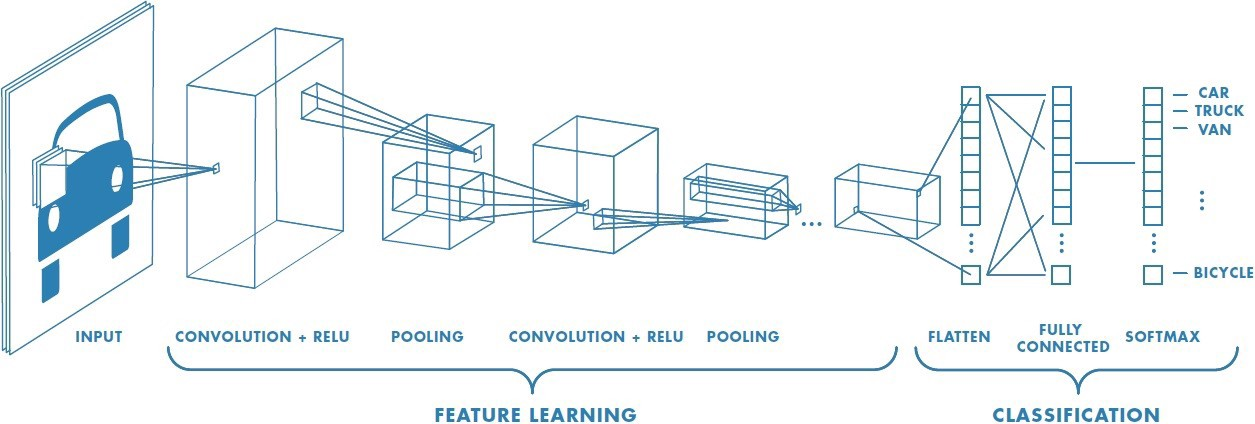
\includegraphics[scale=0.3]{cnn_struct.jpeg}
	\caption{An simplified example of a CNN architecture}
	\label{fig:cnn_struct}
\end{figure}

We will be using transfer learning to reduce the effort involved in training our network. Transfer learning was first proposed in 1993 by Lorien Pratt \cite{Pratt1993} and has been said by Andrew Ng to be the next driver for commercial machine learning success. A comprehensive survey of transfer learning has been completed by Zhuang et al. \cite{Zhuang2019} so we do not detail here all of the developments and differences in various transfer learning algorithms, especially as we plan to take the most basic approach. Whilst many have worked to develop detailed algorithms that take into account the overlap of the source data domain and the target data domain and adjust a network accordingly, we are taking a more simple approach that is discussed in \cref{sub:part_1_genre_predictor} and reusing all but the (dense) classification layers of a network pretrained on ImageNet as the starting point for our training.
% subsection cnn_architecture (end)
\subsection{Existing Datasets} % (fold)
\label{sub:existing_datasets}
The dataset collected by Iwana et al.\cite{KenjiIwana} is the largest, and as far as we can tell only, clean dataset to collate together the book covers of over tens of thousands of books. The dataset exists in two distinct forms; the \emph{BookCover30} dataset and the \emph{Book32} dataset that contain 57,000 and 207,572 records respectively, split across 30 and 32 classes again respectively. Both datasets have the same columns; \emph{Amazon Index, Filename, Image URL, Title, Author, Category Id, Category}. For \emph{BookCover30} there is also a reduced dataset containing just the filename and category ID that can be used for training and testing after image download. A comparison of the volumes, as well as the split between train and test sets, and a key between the category ID and category label can be seen in \cref{tab:book_data_comparison}. In the case that a book belonged to multiple genres, the reported genre was chosen at random.

\begin{table}[]
	\centering
	\begin{tabular}{|l|l|l|l|l|}
	\hline
	\textbf{Label} & \textbf{Category Name}        & \textbf{\begin{tabular}[c]{@{}l@{}}Size\\ Book32\end{tabular}} & \textbf{\begin{tabular}[c]{@{}l@{}}Size \\ BookCover30\\ Training\end{tabular}} & \textbf{\begin{tabular}[c]{@{}l@{}}Size \\ BookCover30\\ Test\end{tabular}} \\ \hline
	0              & Arts \& Photography           & 6,460                                                          & 1710                                                                            & 190                                                                         \\ \hline
	1              & Biographies \& Memoirs        & 4,261                                                          & 1710                                                                            & 190                                                                         \\ \hline
	2              & Business \& Money             & 9,965                                                          & 1710                                                                            & 190                                                                         \\ \hline
	3              & Calendars                     & 2,636                                                          & 1710                                                                            & 190                                                                         \\ \hline
	4              & Children's Books              & 13,605                                                         & 1710                                                                            & 190                                                                         \\ \hline
	5              & Comics \& Graphic Novels      & 3,026                                                          & 1710                                                                            & 190                                                                         \\ \hline
	6              & Computers \& Technology       & 7,979                                                          & 1710                                                                            & 190                                                                         \\ \hline
	7              & Cookbooks, Food \& Wine       & 8,802                                                          & 1710                                                                            & 190                                                                         \\ \hline
	8              & Crafts, Hobbies \& Home       & 9,934                                                          & 1710                                                                            & 190                                                                         \\ \hline
	9              & Christian Books \& Bibles     & 9,139                                                          & 1710                                                                            & 190                                                                         \\ \hline
	10             & Engineering \& Transportation & 2,672                                                          & 1710                                                                            & 190                                                                         \\ \hline
	11             & Health, Fitness \& Dieting    & 11,886                                                         & 1710                                                                            & 190                                                                         \\ \hline
	12             & History                       & 6,807                                                          & 1710                                                                            & 190                                                                         \\ \hline
	13             & Humor \& Entertainment        & 6,896                                                          & 1710                                                                            & 190                                                                         \\ \hline
	14             & Law                           & 7,314                                                          & 1710                                                                            & 190                                                                         \\ \hline
	15             & Literature \& Fiction         & 7,580                                                          & 1710                                                                            & 190                                                                         \\ \hline
	16             & Medical Books                 & 12,089                                                         & 1710                                                                            & 190                                                                         \\ \hline
	17             & Mystery, Thriller \& Suspense & 1,998                                                          & 1710                                                                            & 190                                                                         \\ \hline
	18             & Parenting \& Relationships    & 2,523                                                          & 1710                                                                            & 190                                                                         \\ \hline
	19             & Politics \& Social Sciences   & 3,402                                                          & 1710                                                                            & 190                                                                         \\ \hline
	20             & Reference                     & 3,268                                                          & 1710                                                                            & 190                                                                         \\ \hline
	21             & Religion \& Spirituality      & 7,559                                                          & 1710                                                                            & 190                                                                         \\ \hline
	22             & Romance                       & 4,291                                                          & 1710                                                                            & 190                                                                         \\ \hline
	23             & Science \& Math               & 9,276                                                          & 1710                                                                            & 190                                                                         \\ \hline
	24             & Science Fiction \& Fantasy    & 3,800                                                          & 1710                                                                            & 190                                                                         \\ \hline
	25             & Self-Help                     & 2,703                                                          & 1710                                                                            & 190                                                                         \\ \hline
	26             & Sports \& Outdoors            & 5,968                                                          & 1710                                                                            & 190                                                                         \\ \hline
	27             & Teen \& Young Adult           & 7,489                                                          & 1710                                                                            & 190                                                                         \\ \hline
	28             & Test Preparation              & 2,906                                                          & 1710                                                                            & 190                                                                         \\ \hline
	29             & Travel                        & 18,338                                                         & 1710                                                                            & 190                                                                         \\ \hline
	30             & Gay \& Lesbian                & 1,339                                                          & 0                                                                               & 0                                                                           \\ \hline
	31             & Education \& Teaching         & 1,664                                                          & 0                                                                               & 0                                                                           \\ \hline
	\end{tabular}
	\caption{Comparison of the number of records per category between the Book32 and Book30 training and test sets}
	\label{tab:book_data_comparison}
	\end{table}

The reduced \emph{BookCover30} dataset has already been pre-processed to remove 2 underrepresented classes, and to scale and shape the images; this will likely have to be re-sourced before the processing has taken place as the various CNNs we are going to use have different input shapes. There is also some other issues with the dataset; in particular that no manual filtering was done to ensure that the images are representative of the actual book cover, an example where this is not the case can be seen in \cref{fig:bad_cover}. The data also looks to cover multiple languages so it is possible that there will be duplication of items (although often foreign editions of books have different covers) and this could also lead to additional difficulty if there is a difference in design choices between different countries. Furthermore, this dataset and paper were first published in 2016; while using the same dataset would be useful for comparison it is possible that the same script they used to generate their data could be repurposed to allow for a more up-to-date dataset to be produced, with higher resolution images and a potentially more representative sample of modern books. More discussion on this is repeated in \cref{sub:part_0_data_collection_and_preparation}. 

We mention here for completeness that during our research we did come across a potential alternative source of data, that of the Open Library \cite{openAbout} who as part of the Internet Archive project have the goal to have\emph{"One web page for every book ever published"}. The regular data dumps \cite{openDataDumps} are a possible alternative source to using the Iwana dataset, however this dataset would come with some uncertainty attached. Whilst the volume of records is undoubtedly larger in size, it is not clear without processing all of the records how many of these actually have a genre classification at all, and given that their book covers data dump has not been updated since 2016 it does not provide any more recent data than Iwana's does. We would also be remiss to not mention that as this is an open-source project, the quality of the data itself would be more in question than with the \emph{Book32} records. Finally, it would remove our ability to use Iwana et al's paper as a reference in terms of performance of the networks as not only would the training data itself be vastly different, but the genres are also different in this source.

Overall the \emph{Book32} dataset is the best quality and most label-complete dataset available that we could find, and to produce a new one from scratch even using Open Library as a foundation would take a large amount of work for likely very little gain, so it is this dataset we will use in our work.
\begin{figure}
	\centering
	\captionsetup{justification=centering}
	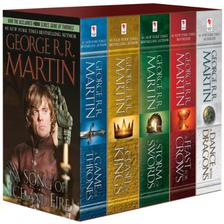
\includegraphics[scale=0.4]{0345535529.jpg}
	\caption{An image in the \emph{BookCover30} dataset showing an anthology box collection rather than the cover}
	\label{fig:bad_cover}
\end{figure}
% subsection existing_datasets (end)
\subsection{Debugging CNNs}
\label{sub:debug_cnn}
CNNs, along with most other deep-learning methods, have been seen for a long time as \emph{black box} methods i.e. it is not possible to understand what a specific neuron or layer within the network is doing. The attitude to black box methods has soured over the years for 2 major reasons. The first being that black box methods are illegal in some fields such as underwriting; a lender must be able to explain to an applicant why they were rejected for a loan, and black box methods do not allow for this. The second is that they are almost impossible to debug and understand where the network may be making an error. Many examples of this were first shown by Nguyen et al \cite{Nguyen} in 2015, where images could be evolved to trick CNNs that return high precision results for obviously garbage images. More recently Su et al. \cite{Su} managed to show that perturbation of even a single pixel in an image can generate a change in the predicted class from otherwise high performing classifiers. These examples, combined with a drive for more explainable AI, has led to a few key developments in the debugging of CNNs via representative visualisation. 

In 2018 Qin et al. \cite{Qin2018a} produced a survey of the major visualisation methods and whilst there has been some developments, mostly in the implementation of these methods in common software packages, their work remains a good summary of the state of the work. They call out four key visualisation methods:
\begin{enumerate}
	\item Activation maximisation - A visualised image is generated such that it maximises a specific neuron's activation.
	\item DeconNet - Uses an inverted CNN structure to identify the pattern in the input image that triggers specific neuron activation.
	\item Network Inversion - Recreates an image based on the input image from a specific layer, helping identify what information is preserved by this layer.
	\item Network dissection  - Applies semantic concepts to each neuron such as scene, material, object etc.
\end{enumerate}
For the purpose of this work we focus only on activation maximisation as this is what we plan to use to generate representative images of some of the genres. 

Activation maximisation was proposed by Erhan et al. \cite{erhan2009} in 2009 and the idea itself is quite simple; iteratively perturbate an image to maximise the activation of a given neuron. The resultant image then represents what that neuron has learned. The actual algorithm uses backpropagation instead of perturbation to improve the synthesised image over many iterations. Compared to normal backpropagation where we calculate the change in the network error with respect to each weight and bias and use that to update the values, here we calculate the change in activation with respect to the input and use this as the base for our update rule:
\begin{equation}
	input_{t} = input_{t-1} - \eta\times\frac{\partial ActivationMaximisationLoss}{\partial input_{t-1}}
\end{equation} 
where $ActivationMaximisationLoss$ is some loss measure that decreases as the activation increases, and $\eta$ is a learning rate. We stop when the activation of the neuron cannot be increased further. This can be applied to almost any neuron in the network with no alteration to the structure except for those in the final layer. The final layer activation function, the transformation applied to the inputs of the neuron, must be changed from the pre-existing SoftMax ($\sigma$) as defined in \cref{eq:softmax}, which takes a vector of activations for the $K$ output classes and normalises them to be between 0 and 1 with a sum of 1, and be replaced with a linear function instead (often just the linear sum of inputs is used). The reason for this is that to maximise the output of a SoftMax function for a single neuron, it is possible to minimise the values of the other neurons. This leads to a case where the generated image would not be representative of our target class, but just be more representative than it is of the other classes. By using the unbounded linear function we can continue to apply updates to the input until we see little to no increase in the activation for our target neuron, irrespective of the other class activations.

\begin{equation}
	\sigma(\vec{x})_i = \frac{e^{x_i}}{\sum_{j=1}^{K}e^{x_j}}
	\label{eq:softmax}
\end{equation}

Often, this approach is taken together with some form of normalisation to improve the interpretability of these images. As mentioned, pictures that are composed entirely of noise can trigger activation in the output neurons in a network with high certainty, so these normalisation methods are applied to reduce the production of these types of images and return more visually understandable results. Some of these normalisations, such as $l_2$ decay (which usually uses the sum of squared weight, but pixel values in this case) are used to prevent a few pixels dominating the image, or applying a Gaussian Blur can be done to ensure that no area of the image has too high an information frequency.

The final extension to this work is that of \emph{Deep Generative Network Activation Maximization} (DGN-AM)\cite{Nguyena} which adds in a generative network, a network with the goal of producing an item of the specified class rather than to classify an object into a class, to produce more realistic images as opposed to the abstract ones often produced by activation maximisation. They were first used in 2016 and have shown greatly improved results, but also require greatly increased network complexity and training time. DGN-AMs have also been shown to provide worse outputs when the generative network is not the same architecture as the CNN and so multiple generative networks would need to be created for this work which would be far too computationally expensive; as such we chose to not use them within this work. An example taken from Qin's survey is shown in \cref{fig:am_dgnam} highlighting the huge change that using DGN-AMs produce. 

\begin{figure}
	\centering
	\captionsetup{justification=centering}
	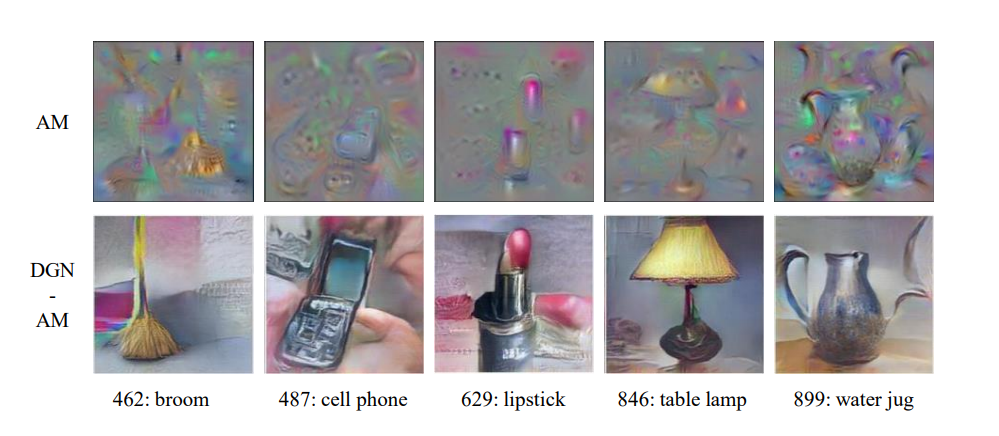
\includegraphics[scale=0.4]{am_vs_dgnam.PNG}
	\caption{Activation Maximization vs Deep Generative Network Activation Maximization from "How convolutional neural network see the world - A survey of convolutional neural network visualization methods" by Qin et al, 2018}
	\label{fig:am_dgnam}
\end{figure}
% section lit_rev (end)
\section{Proposal} % (fold)
\label{sec:proposal}
\subsection{Planned work}
The proposed work is to be completed in 3 distinct parts, starting with the work detailed in \cref{sub:part_0_data_collection_and_preparation} focusing on the collection and reprocessing of the data first generated by Iwana et al. \cite{KenjiIwana} to ensure completeness and correctness. We then in \cref{sub:part_1_genre_predictor} propose to reproduce the work of Iwana et al. and then develop this further using recent advances in CNN architecture. Finally \cref{sub:part_3_inverting_the_network} discusses the plans to use activation maximisation on the CNN to produce images based on the output class.
\subsubsection{Part 1: Data Collection and Preparation} % (fold)
\label{sub:part_0_data_collection_and_preparation}
The work first produced by Iwana\cite{KenjiIwana} uses a reduced dataset of 57,000 book covers that span 30 classes with 1,900 records each. We will first step back to the \emph{Book32} dataset to have available to us the full use of 207,572 books; we will download and ensure via some manual testing that the URLs of the images are still the correct ones from the time of writing.  

At this stage any images will all be pre-processed including scaling to be a sensible size. The complexity is that of the shape of book covers in general, whilst there is some standardisation across the industry, is not fixed as shown in \cref{fig:book_cover_sizes} and specific genres of books such as cookbooks are likely to take a different shape due to their usage and content. This means that by scaling the images we are likely to impact some classes more than others. Analysis will be conducted to identify the distribution of shapes and if this varies by class, as well as a review of various methods used within the literature to approach such a problem. In particular an approach similar to the NIST dataset as reproduced by Cohen at al. \cite{Cohena} could be used with some adaptations for colour images.

Once this has been completed we will need to re-sample the dataset down to the same size as the original work, however we may not use the exact same subset of books they selected if we believe we can responsibly remove unrepresentative images such as the one displayed in \cref{fig:bad_cover}. This will lead to an inability for exact comparison between our work and that of Iwana, however it should help improve the accuracy of the model by removing non-representative training and test data. Where possible the same records will be used within the training and test sets, and only those that we identify to be non-standard will be swapped for another record.
\begin{figure}
	\centering
	\captionsetup{justification=centering,margin=2cm}
	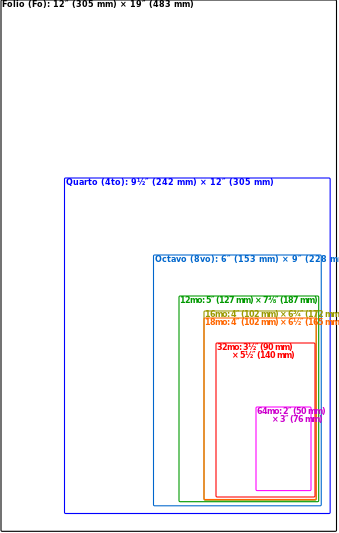
\includegraphics[scale=0.5]{Comparison_book_sizes}
	\caption{Comparison of book sizes based on \cite{AmericanLibraryAssociation.CommitteeonLibraryTerminology.1971}\\
		\footnotesize{By Cmglee - Own work, CC BY-SA 3.0, https://commons.wikimedia.org/w/index.php?curid=15264645}}
	\label{fig:book_cover_sizes}
\end{figure}
% subsection part_0_data_collection_and_preparation (end)
\subsubsection{Part 2: Genre Predictor via Transfer Learning} % (fold)
\label{sub:part_1_genre_predictor}
In their work, Iwana et al\cite{KenjiIwana} trained 2 CNNs (LeNet and AlexNet) on the training set and report the Top 1 and Top 3 predicted class accuracy by book genre on the test set. We will attempt to reproduce the results achieved by them using AlexNet on our adjusted dataset and just use the LeNet results for an approximate comparison. We will use the same method as they did to train AlexNet i.e. apply transfer learning to a pre-trained version of the network on the ImageNet dataset, removing the classification layers of the network, those densely connected non-convolutional layers, including the  final 1000 neuron dense layer (representing the 1000 classes) and replace it with a similar network ending with a layer of 30 densely connected neurons instead, 1 for each of our genres, freezing the weights of the feature-extraction part of the network before beginning training.

Once a baseline has been established we will intended to improve the per-class accuracy by using some of the newer architectures as shown in \cref{fig:cnn_history}, namely Inception-ResnetV2 and a ResNeXt, and see if these yield better results. We will also look at using any of the techniques in the literature for differing shaped input images at this point to see if it is possible to provide not just the cover image to the network, but also information about the shape and size of it as well in the chance that this may improve accuracy. We again will use transfer learning here to greatly reduce the computational cost and time to train these models. The specific details of these CNN architectures will be discussed more within the work itself. 

\begin{figure}
	\centering
	\captionsetup{justification=centering,margin=2cm}
	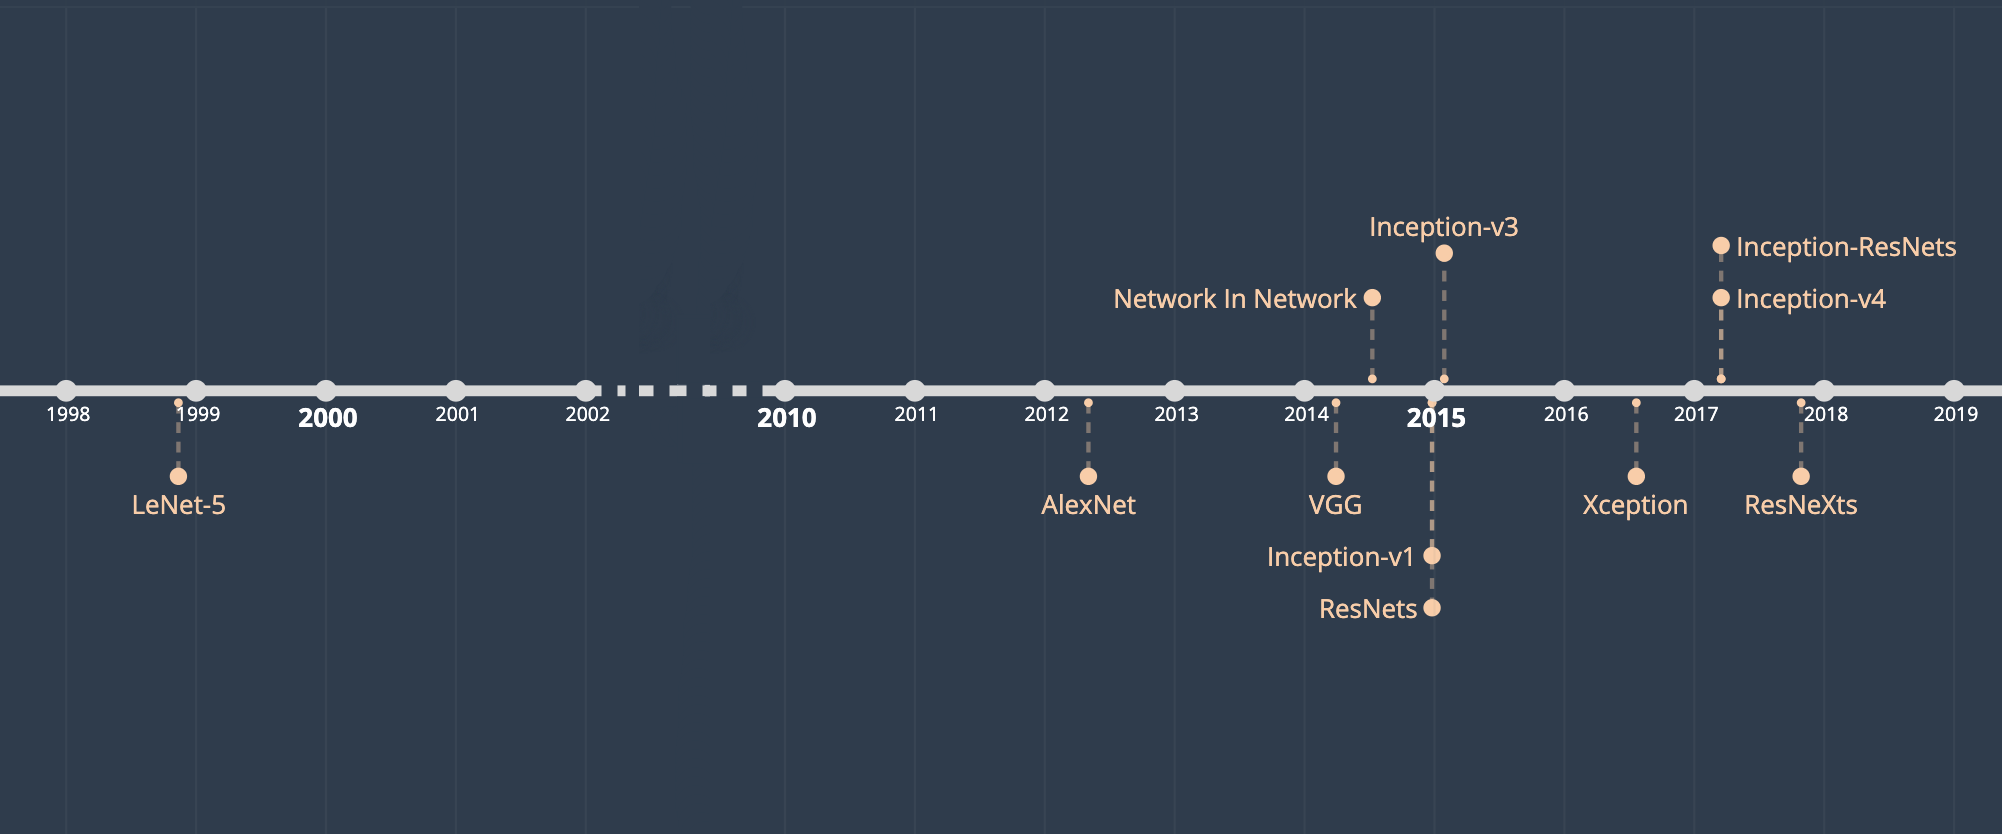
\includegraphics[scale=0.22]{CNN_HISTORY.png}
	\caption{Key CNN architectures and their year of publication\cite{Karim2019}}
	\label{fig:cnn_history}
\end{figure}
% subsection part_1_genre_predictor (end) 
\subsubsection{Part 3: Feature Visualisation}
\label{sub:part_3_inverting_the_network}
Once we have compared the performance of the different CNN architectures on the dataset we will attempt to use activation maximisation as discussed in \cref{sub:debug_cnn} with the network and instead of predicting the genre based on an image, it will produce an image based on a requested genre. This is sometimes also referred to as feature visualisation, although rather than individual features we are trying to reproduce a whole input. We will only take the best and worst 2-3 performing genres based on the previous stage to attempt this for.

To do this we propose the use of the relatively new and still under active development python package \emph{tf-keras-vis} \cite{keras-vis}. This package offers 2 key feature visualisation techniques; activation maximisation for filter layers and final output layers, and attention (i.e. what area of the image is driving the output class the network has predicted). Using this package we should be able to produce images that maximise the activation of our target class neuron. As mentioned in \cref{sub:debug_cnn} it is probable that these images will be abstract and may be entirely uninterpretable, but they may shed some insight on how specific genres are easier to predict than others and so we believe it adds value to the project.

\subsection{Hardware and Software}
Even using transfer learning, the amount of epochs the networks will have to train for to get a reasonable accuracy is still likely to be quite high, and as these are complex deep networks this will take a lot of time. Because of this we propose the use of Google Colab \cite{Google} to enable the use of GPUs, and potentially Tensor Processing Units (TPUs), for an order of magnitude speed up in the training of these networks. There is a limit on the amount of time a single session can run for, and there is no guarantee on the specific G/TPU brand/architecture that will be used, but without this or an approach similar it is unlikely that we posses the computing power to complete the work. As a point of note, TPUs are likely to offer a faster training however require a non-trivial amount of additional setup and so the choice to use them will be evaluated on a case by case basis. Because of this it is not possible to specify the exact hardware that we will use for this work.

For software, the majority of the work in terms of downloading, pre-processing, modelling, evaluations, and visualising features will be done in python using Tensorflow 2.x with a Keras backend, with heavy support from both the sklearn package and the aforementioned tf-keras-vis package. Visualisation outside of features may be done using R after some pre-analysis in python due to the extensive variety of libraries that support the production of graphics in R compared to python, as well as our own familiarity with the language.  
% section proposal (end)
\section{Conclusion} % (fold)
\label{sec:conclusion}
In this work we have laid out a problem which can be summarised as \emph{Can a CNN judge a book by its cover} and highlighted some of the previous work already completed in this space, namely that of Iwana et al. We discussed the existing available datasets, known as \emph{BookCover30} and \emph{Book32}, and explored some of the limitations this dataset currently has and we may potentially wish to address. Following this we laid out a 3 stage plan for trying to answer the question, starting with data collection and pre-processing, then using transfer learning to train high-performing CNN architectures for this problem and evaluating their performance. Finally we spoke of plans to use feature visualisation techniques to produce idealised covers for the most and least accurate genres from our models. Overall the proposed work should produce, as far as we can tell at time of writing, the only follow-up work to the Iwana paper and update their work using the more recent developments in CNN architecture and computing power.
% section conclusion (end)
%\nocite{*}
\bibliographystyle{ieeetran}
\bibliography{BBK_MSc_Project} 
\end{document}